\section{État de l'art}
\label{sec:etat_art}

    \subsection{Numérisation de documents}
    \label{subsec:numerisation}
    Même si le sujet se centre sur la consultation de documents numérisés, il est intéressant d’avoir un aperçu des solutions
    qui existent aujourd’hui pour pouvoir numériser des documents anciens. En effet un nombre non négligeable d’entreprises
    proposent aujourd’hui la numérisation de nombreux types de documents.

        \subsubsection{Arkhenum}
        \label{subsubsec:arkhenum}
        Arkhenum est une entreprise spécialisée dans la numérisation de documents anciens datant du Vème au XXème siècle.
        Les types de documents numérisés sont très variés : cartes, plans, archives (registres d'état civil, paroissiaux,
        militaires, etc), affiches, livres, manuscrits, etc. Arkhenum travaille à la demande de bibliotèques, de centres d'archives,
        de cinématèques ou bien de musées. L'idée est d'utiliser la numérisation afin de préserver et de diffuser ces documents.

        La valeur d'Arkhénum est avant tout la préservation des documents, un soin particulier est donc apporté à la manipulation
        à des documents, le protocole de numérisation est donc adapté : pas de vitre de numérisation, ouverture des reliures limitée
        120\degree, utilisation de gants en coton. Arkhénum mise également sur la haute qualité des numérisations en adaptant l'éclairage,
        le cadrage et en appliquant des traitements de correction des courbures.

        Arkhenum se pose en tant que service de numérisation plutôt que plateforme de diffusion. C’est le client à l’origine de la
        numérisation qui se charge de la diffusion des documents numérisés. L'activité de notre projet se situe donc à posteriori de l'activité d'Arkhénum.

        \subsubsection{Azentis}
        \label{subsubsec:azentis}
        Azentis a une activité beaucoup plus large. C’est une entreprise travaillant sur la totalité du processus de conservation de documents,
        de la  numérisation à la diffusion. Les documents numérisés sont de types variés : archives (registres d'état civil, paroissiaux,
        parchemins, livres anciens, livres, presse ancienne, cadastres), documents (techniques, commerciaux, personnels, comptables, logistiques,
        d'urbanisme, etc), photos, plans.

        Azentis est également présent sur la diffusion. En effet, elle développe des solutions de consultation de documents numérisés ayant
        des fonctions de recherches par mot clé. Cependant, ces solutions de consultation sont développées au cas par cas, pour chacun de ses clients.
        Il n'y a pas de plateforme publique de centralisation des documents numérisés.

    \subsection{Consultation de documents}
    \label{subsec:consultation}
    Il n’existe pas de plateforme dédiée qui référence et permette d’accéder à des documents de la presse ancienne. Cependant on peut constater
    de plus en plus un gain d’intérêt (notamment suite à des évènements comme les 100 ans de la Grande Guerre) d’accéder à des documents anciens
    qui peuvent être des actes de naissance, des registres d’état civil, des registres matricules … et plusieurs plateformes ont vu le jour
    ces dernières années, permettant de consulter des documents de ce genre.

        \subsubsection{Archives des Yvelines}
        \label{subsubsec:yvelines}
        “Archives Yvelines” est une plate-forme d’archivage et de consultation de documents antérieures à 1790 concernant les communes d’Yvelines,
        rassemblées pendant la Révolution. La plate-forme comporte de près de 2 167 410 pages parmi lesquels  des archives publiques et privées,
        ouvrages de bibliothèques, titres de presse locale, photographies et cartes postales, maquettes, pages numérisées, documents communiqués
        en salle de lecture, expositions virtuelles...

        La plate-forme des archives d’Yvelines permet de faire une recherche plus ou moins affinée en fonction d’une thématique (registres paroissiaux,
        recencement de population, répertoires de notaires, presse ancienne,…) ou de la commune.

        Par exemple, pour une recherche dans les registres paroissiaux et d’état civil (illustrée par la figure ci contre), il est possible de choisir
        plusieurs critères d’affinement de la recherche comme la cote, le type d’acte, la période...

        La recherche par commune donne accès à tous les différents documents d’une commune.

        Après accès au document, il est possible d’effectuer plusieurs actions  en fonction du type de document. Par exemple pour le documents numérisés,
        les principales actions sur le document sont le zoom, le téléchargement, la récupération du lien, l’ajout dans un panier, le signalement d’une erreur,
        l’annotation et l’impression (confère la figure ci-dessous).

        Il existe certains documents comme les fiches concernant les navires de guerre (figure ci-dessous) où il n’est possible d’effectuer aucune action pendant la consultation.

       Enfin, le dernier type de consultation des documents concerne la presse ancienne. Il est possible d’effectuer une recherche plein texte sur le document.

        \subsubsection{Mémoire des hommes}
        \label{subsubsec:memoire}
        “Mémoire des hommes” est aussi une plate-forme de consultation d’anciens documents  qui a été inaugurée en 2003. Elle comporte essentiellement
        des fiches numérisées concernant les militaires français acteurs des conflits tels que la première et seconde guerre mondiale, la guerre d’Indochine,
        la guerre de Corée, ou encore la guerre d’Algérie.

        Le site “Mémoire des hommes” permet d’effectuer une recherche soit grâce aux indexations réalisées à l’aide des annotations des utilisateurs,
        soit par thématique de guerre. Il est possible d’affiner la recherche avec des informations concernant la personne telles que le nom,
        la date de naissance, le lieu de naissance, le département, ...

        Les actions réalisables sur les documents sont identiques à celles de la plate-forme des archives d’Yvelines, les deux plateformes utilisant
        le même outil pour la visualisation de documents.

        Le site ‘Mémoire des hommes’ possède une petite particularité qui est la cartographie pour certaines guerre comme la guerre de Corée;
        cartographie sur laquelle et localisée chacune des batailles de la guerre, la période et le nombre de décès.

        \subsubsection{Numdam}
        \label{subsubsec:numdam}
        C’est un programme de la Cellule de coordination documentaire nationale pour les mathématiques (Mathdoc) soutenant des revues de
        mathématiques en rendant leurs archives consultable sur internet. Les revues sont scannées en haut définition et mises à disposition
        en format djvu ou pdf. Le texte des pdfs est protégé contre la copie mais on peut cependant faire une recherche de mots dessus.
        On note la présence du format djvu adapté aux liseuses électroniques, ce dernier n’est pas protégé contre la copie du texte.
        La bibliothèque est relativement pauvre avec une collection de 36 journaux, 32 séminaires et 5 mémoires.

        \subsubsection{Gallica}
        \label{subsubsec:gallica}
        C’est la bibliothèque numérique de la Bibliothèque nationale de France, elle est en ligne depuis 1997. La bibliothèque
        est très riche de contenu avec aujourd’hui plusieurs millions de documents et chaque semaine des milliers de nouveautés.
        On peut consulter les œuvres directement sur le site, nous avons accès à tout un panel de commandes pour naviguer dans l’ouvrage:
        flèches suivant/précèdent, zoom, rotation, plein écran, recherche sur le texte, mode d’affichage, téléchargement, partage, signaler une anomalie.
        On a accès à des légendes en rapport avec l’œuvre et dans le même panel au texte où l’on peut effectuer une recherche plein texte. Cependant,
        le texte, reconnu avec un OCR, est parfois inexact. Gallica informe avoir eu recourt à deux types d’OCR, un OCR brut sans intervention humaine
        ou un OCR avec montée en qualité du texte ou celui-ci est amélioré par une correction manuel. On peut ainsi attendre un taux qualité cible de
        96 à 99.9\% avec l’OCR le plus qualitatif.

        \begin{figure}[ht!]
            \centering
            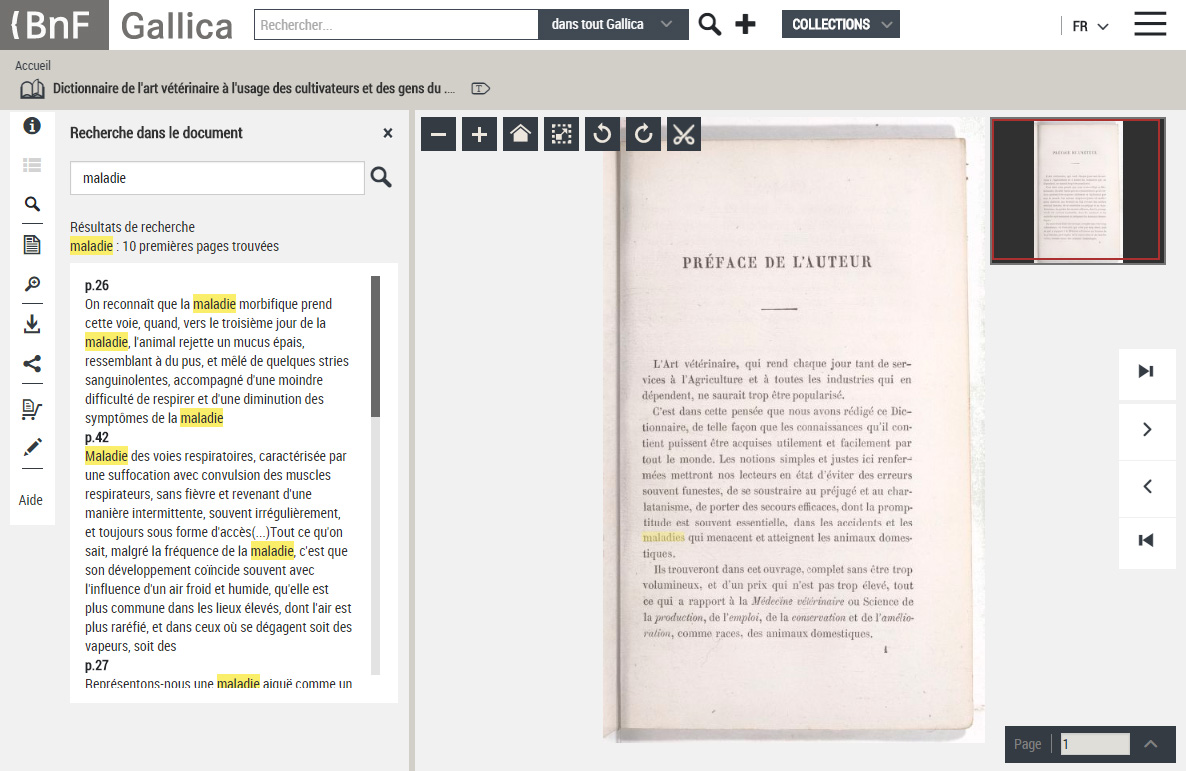
\includegraphics[width=1\textwidth]{figure/screenshot_gallica.jpg}
            \caption{Capture d'écran du moteur de recherche Gallica}
            \label{fig:gallica}
        \end{figure}

        Pour le téléchargement, on peut télécharger le document en entier ou une sélection du document soit en pdf, soit en jpeg pour la page en cours.
        Les options de consultation évoluent aussi en fonction du type de texte, ainsi la légende, recherche dans le document ou table des matières
        ne sont pas disponible pour tous les ouvrages. Pour les manuscrits par exemple on n’aura accès au texte plein et pour les revues souvent juste
        la table des matières. Outre la visionneuse disponible sur le site web, Gallica propose des applications mobiles sur Google Play et App Store.
